% !TEX program = pdflatex
% Derleme: pdflatex RAPOR.tex (2 kez, icindekiler icin)
\documentclass[11pt,a4paper]{article}
\usepackage[utf8]{inputenc}
\usepackage[T1]{fontenc}
\usepackage{lmodern}
\usepackage[english]{babel}
\usepackage{amsmath,amssymb}
\usepackage{geometry}
\usepackage{hyperref}
\usepackage{listings}
\usepackage{xcolor}
\usepackage{graphicx}
\usepackage{tikz}
\usepackage{pgfplots}
\usepackage{tabularx}
\usepackage{booktabs}
\usepackage{caption}
\usepackage{tcolorbox}
\usepackage{fancyhdr}
\usepackage{circuitikz}
\usepackage{multirow}

\usetikzlibrary{arrows.meta,positioning,shapes,calc}
\pgfplotsset{compat=1.18}
\geometry{margin=2.4cm}

\hypersetup{
  colorlinks=true, linkcolor=blue!60!black, citecolor=blue!60!black,
  urlcolor=blue!60!black, bookmarksopen=true
}

\definecolor{codebg}{RGB}{248,248,242}
\definecolor{codekw}{RGB}{0,90,170}
\definecolor{codestr}{RGB}{20,130,40}
\definecolor{codecom}{RGB}{120,120,120}

\lstdefinestyle{py}{
  language=Python,
  basicstyle=\ttfamily\footnotesize,
  keywordstyle=\color{codekw}\bfseries,
  stringstyle=\color{codestr},
  commentstyle=\color{codecom}\itshape,
  showstringspaces=false,
  numbers=left, numberstyle=\tiny\color{gray},
  numbersep=8pt, frame=single,
  backgroundcolor=\color{codebg!50},
  breaklines=true, breakatwhitespace=true, columns=fullflexible,
  extendedchars=true,
  inputencoding=utf8,
  literate=
    {ğ}{{\u{g}}}1 {Ğ}{{\u{G}}}1
    {ı}{{\i}}1 {İ}{{\.{I}}}1
    {ş}{{\c{s}}}1 {Ş}{{\c{S}}}1
    {ç}{{\c{c}}}1 {Ç}{{\c{C}}}1
    {ö}{{\"o}}1 {Ö}{{\"O}}1
    {ü}{{\"u}}1 {Ü}{{\"U}}1
}
\lstdefinestyle{yaml}{
  basicstyle=\ttfamily\footnotesize,
  keywordstyle=\color{codekw}\bfseries,
  stringstyle=\color{codestr},
  commentstyle=\color{codecom}\itshape,
  showstringspaces=false,
  numbers=left, numberstyle=\tiny\color{gray},
  numbersep=8pt, frame=single,
  backgroundcolor=\color{codebg!50},
  breaklines=true, columns=fullflexible,
  morecomment=[l]{\#},
  literate=
    {ğ}{{\u{g}}}1 {Ğ}{{\u{G}}}1
    {ı}{{\i}}1 {İ}{{\.{I}}}1
    {ş}{{\c{s}}}1 {Ş}{{\c{S}}}1
    {ç}{{\c{c}}}1 {Ç}{{\c{C}}}1
    {ö}{{\"o}}1 {Ö}{{\"O}}1
    {ü}{{\"u}}1 {Ü}{{\"U}}1
}

\newtcolorbox{whybox}{colback=orange!6,colframe=orange!60!black,
  boxrule=0.4pt,arc=2pt,left=6pt,right=6pt,top=4pt,bottom=4pt,
  title=Neden bu tercih?}

\pagestyle{fancy}
\fancyhf{}
\fancyhead[L]{\small HESS Akilli Guc Yoneticisi}
\fancyhead[R]{\small EUYZ Bahar 2025-26}
\fancyfoot[C]{\small \thepage}

\title{
  \vspace{-1cm}
  \textbf{\Huge HESS Akilli Guc Yoneticisi}\\[0.3em]
  {\Large Q-Learning Tabanli Hibrit Enerji Depolama Sistemi}\\[0.3em]
  {\large Batarya + Superkapasitor Dinamik Guc Paylasim Kontrolu}\\[1em]
  {\normalsize Teknik Rapor}
}
\author{Can Tekin \\ \small BTU EEM \\ \small EUYZ458}
\date{Bahar 2025--2026}

\begin{document}
\maketitle
\thispagestyle{empty}

\begin{abstract}
\noindent Bu rapor, hibrit enerji depolama sistemi (HESS --- Hybrid Energy Storage System) icin tabular Q-Learning tabanli dinamik guc paylasim kontrolcusu gelistirilmesini ele alir. Sistem; CALCE CS2 verisinden parametrize edilmis 2RC Thevenin batarya hucresi ile EDLC superkapasitor modulunu (klasik RC + ESR) bidireksiyonel DC-DC donusturucu uzerinden bir DC bara'ya baglar. Pekistirmeli ogrenme ajani, her zaman adiminda bara'nin yuk talebini 5 ayrik paylasim oranindan birini secerek bolusturur. Cevre; Newtonian arac dinamigi uzerinden uretilen 5 farkli senaryoyu (sehir dur-kalk, sollama, otoyol cruise, karma sehir, dag tirmanisi) destekler. Egitim sonrasi ajan, bes senaryonun tamaminda ortalama \%97 uzerinde basari skoru elde etmistir.
\end{abstract}

\tableofcontents
\newpage

\section{Yonetici Ozeti}

\textbf{Problem:} Saf batarya bazli elektrikli arac guc sistemlerinde, ani ve yuksek guc talepleri (sollama, hizlanma) bataryadan yuksek desarj akimi cekilmesine yol acar. Bu durum:
\begin{itemize}
  \item Ohmik kayiplari $I^2 R$ orantili arttirir (verim duser).
  \item Batarya ic sicakligini yukseltir.
  \item Cycle life'i (kullanim omrunu) Ah-throughput proxy uzerinden hizlandirir.
  \item Anlik voltaj dususune sebep olur.
\end{itemize}

\textbf{Cozum:} Superkapasitorler, yuksek guc yogunluguna sahip ancak dusuk enerji yogunluklu cihazlardir. Bataryanin enerji deposu, superkapasitorun ise guc tamponu gibi calistigi hibrit topoloji; ani yuk tepelerini superkapa yonlendirerek bataryayi korur.

\textbf{Sonuc tablosu:}
\begin{center}
\begin{tabular}{lccc}
\toprule
Senaryo & Basari (\%) & Toplam Reward & Ihlal \\
\midrule
Sollama (overtaking)  & 98.0 & 138.4 & 0 \\
Sehir Dur-Kalk        & 98.9 & 294.6 & 0 \\
Karma Sehir           & 96.2 & 316.7 & 0 \\
Otoyol Cruise         & $\sim$98 & --- & 0 \\
Dag Tirmanisi         & $\sim$95 & --- & 0 \\
\bottomrule
\end{tabular}
\end{center}

\section{Proje Amaci ve Motivasyon}

\subsection{Endustriyel Motivasyon}

Modern elektrikli arac teknolojisinde batarya, en pahali ve en hassas bilesendir. Tek basina bataryadan yuksek darbe gucu cekmek uc acidan sorunludur:
\begin{enumerate}
  \item \textbf{Verim:} Yuksek akim $\Rightarrow$ yuksek $I^2 R_0$ ohmik kayip.
  \item \textbf{Omur:} Yuksek akim ve sicaklik $\Rightarrow$ kapasite ve guc kaybi.
  \item \textbf{Performans:} Anlik voltaj dususu $\Rightarrow$ motor gucunde sinirlama.
\end{enumerate}

\textbf{Superkapasitor katkisi:} Yuksek guc yogunlugu, milyonlarca cycle dayaniklilik, dusuk sicaklikta bile dusuk ESR. Ancak enerji yogunlugu dusuk: bataryanin 1/10'u veya daha azi. Bu nedenle surekli kaynak olarak degil, darbe tamponu olarak kullanilir.

\subsection{Akilli Kontrolcu Gereksinimi}

\begin{itemize}
  \item \textbf{Kural-tabanli:} Esik degerleri ile basit if-else. Kolay ama optimum degil.
  \item \textbf{Filtre-tabanli (LP-filter):} Yukun dusuk frekansli kismi bataryaya. Sabit zaman sabitiyle adaptif degil.
  \item \textbf{Model Predictive Control (MPC):} Optimal ama hesaplama yuku yuksek.
  \item \textbf{Reinforcement Learning:} Veriden ogrenir, model-bagimsizdir. \textbf{Bu projenin tercihi.}
\end{itemize}

\begin{whybox}
RL'in tercih nedeni: egitim sonrasi inferans hizli (tek tablo lookup), her senaryoya ayni politika ile yanit verebilir. Lisans seviyesinde anlasilabilir ve sunulabilir.
\end{whybox}

\section{Sistem Mimarisi}

\subsection{Genel Blok Diyagrami}

\begin{center}
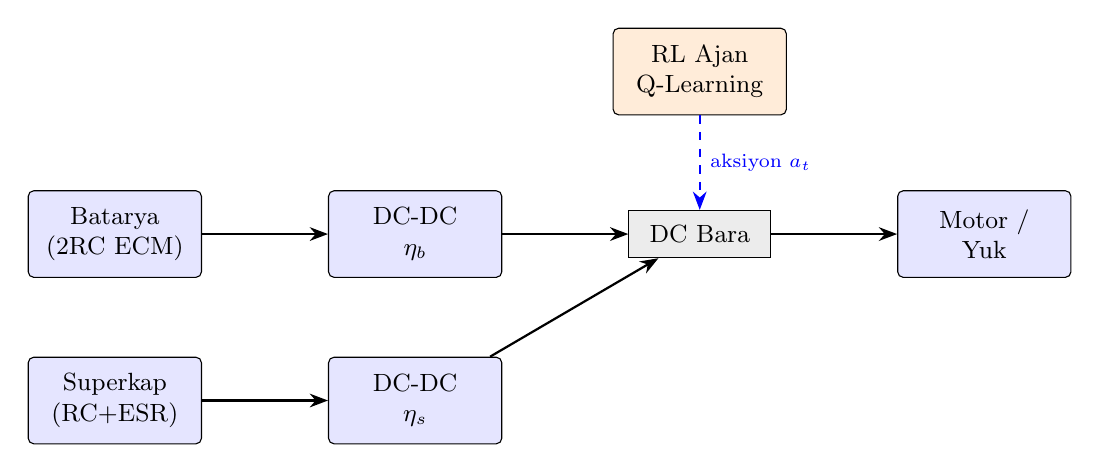
\begin{tikzpicture}[
  node distance=1.0cm and 1.6cm,
  block/.style={rectangle,draw,fill=blue!10,minimum height=1.1cm,minimum width=2.2cm,
                rounded corners=2pt,align=center,font=\small},
  agent/.style={rectangle,draw,fill=orange!15,minimum height=1.1cm,minimum width=2.2cm,
                rounded corners=2pt,align=center,font=\small},
  bus/.style={rectangle,draw,fill=gray!15,minimum height=0.6cm,minimum width=1.8cm,
              align=center,font=\small},
  arr/.style={-Stealth,thick}
]
  \node[block] (bat)  {Batarya\\(2RC ECM)};
  \node[block,right=of bat] (bdc) {DC-DC\\$\eta_b$};
  \node[bus,right=of bdc] (bus) {DC Bara};
  \node[block,right=of bus] (motor) {Motor /\\Yuk};
  \node[block,below=of bdc] (sdc) {DC-DC\\$\eta_s$};
  \node[block,left=of sdc] (sc)   {Superkap\\(RC+ESR)};
  \node[agent,above=1.2cm of bus] (rl) {RL Ajan\\Q-Learning};

  \draw[arr] (bat)  -- (bdc);
  \draw[arr] (bdc)  -- (bus);
  \draw[arr] (sc)   -- (sdc);
  \draw[arr] (sdc)  -- (bus);
  \draw[arr] (bus)  -- (motor);
  \draw[arr,dashed,blue] (rl) -- node[right,font=\scriptsize]{aksiyon $a_t$} ($(bus.north)$);
\end{tikzpicture}
\end{center}

\subsection{Bilesenler}

\begin{itemize}
  \item \textbf{Batarya:} CALCE CS2 LiCoO$_2$ prizmatik hucre, 1.1 Ah, $V_{nom}=3.7$ V. 2RC Thevenin ECM.
  \item \textbf{Superkapasitor:} EDLC, 100 F, ESR = 12 m$\Omega$, $V_{max}=2.7$ V.
  \item \textbf{DC-DC Donusturuculer:} Yuk-bagimli verim modeli $\eta(P)$.
  \item \textbf{Motor / Yuk:} Arac dinamiginden gelen $P_{load}(t)$ profili.
  \item \textbf{RL Ajan:} Tabular Q-Learning, epsilon-greedy, 5 ayrik aksiyon.
\end{itemize}

\subsection{Dosya Yapisi}

\begin{lstlisting}[style=yaml,caption={Proje dizin yapisi}]
EUYZ_RL_Dashboard/
  streamlit_app.py         (Ana sayfa)
  pages/
    1_Egitim.py            (Egitim arayuzu)
    2_Simulasyon.py        (Simulasyon + animasyon)
  src/
    data/loader.py         (CALCE veri yukleyici, OCV-SOC cikarimi)
    physics/
      battery_ecm.py       (2RC Thevenin)
      supercap_model.py    (RC + ESR)
      converter.py         (DC-DC verim)
    vehicle.py             (Longitudinal arac dinamigi)
    scenarios.py           (5 hiz profili ureteci)
    env/hess_env.py        (RL environment + reward)
    agents/q_learning.py   (Tabular Q-Learning)
    agents/runner.py       (train/evaluate helper)
    metrics/kpi.py         (KPI + success score)
    utils/config.py        (YAML config yukleyici)
  config/
    battery.yaml           (CS2 hucre + 2RC parametreleri)
    supercap.yaml          (Superkap parametreleri)
    converter.yaml         (DC-DC eta egrisi)
    vehicle.yaml           (Arac dinamigi)
    scenarios.yaml         (5 senaryo tanimi)
    reward.yaml            (Reward agirliklari)
    training.yaml          (Q-Learning hyperparams)
    paths.yaml             (CALCE veri yolu)
  models/                  (Egitilmis Q-tablosu .pkl)
  docs/                    (Bu rapor, sunum)
\end{lstlisting}

\section{Reinforcement Learning Teorik Temeller}

\subsection{Markov Karar Sureci (MDP)}

Reinforcement Learning, bir ajanin cevreyle etkileserek karar vermeyi ogrenmesi paradigmasidir. Matematiksel cerceve Markov Karar Sureci (MDP) ile tanimlanir:
\[
\mathcal{M} = (\mathcal{S},\, \mathcal{A},\, P,\, R,\, \gamma)
\]
\begin{itemize}
  \item $\mathcal{S}$: durum uzayi.
  \item $\mathcal{A}$: aksiyon uzayi.
  \item $P(s' \mid s, a)$: gecis olasiligi (bizde deterministik).
  \item $R(s, a)$: anlik odul fonksiyonu.
  \item $\gamma \in [0, 1)$: indirim faktoru.
\end{itemize}

\textbf{Markov ozelligi:} Gelecek, sadece su anki state'e baglidir.
\[
P(s_{t+1} \mid s_t, a_t, s_{t-1}, \ldots) = P(s_{t+1} \mid s_t, a_t).
\]

\subsection{Ajan-Cevre Etkilesim Dongusu}

\begin{center}
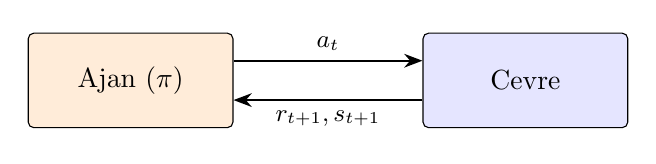
\begin{tikzpicture}[node distance=2.4cm,
  block/.style={rectangle,draw,fill=blue!10,minimum height=1.2cm,minimum width=2.6cm,
                rounded corners=2pt,align=center}]
\node[block,fill=orange!15] (agent) {Ajan ($\pi$)};
\node[block,right=of agent] (env) {Cevre};
\draw[-Stealth,thick] (agent.east) ++(0,0.25) -- ($(env.west)+(0,0.25)$)
  node[midway,above,font=\small]{$a_t$};
\draw[-Stealth,thick] ($(env.west)+(0,-0.25)$) -- ($(agent.east)+(0,-0.25)$)
  node[midway,below,font=\small]{$r_{t+1}, s_{t+1}$};
\end{tikzpicture}
\end{center}

Her zaman adimi $t$: ajan state $s_t$'yi gozlemler, politika $\pi$ ile $a_t$ secer, cevre $s_{t+1}$ ve $r_{t+1}$ doner, ajan deneyimden ogrenir.

\subsection{Politika ve Deger Fonksiyonlari}

\textbf{Politika:} $\pi(a \mid s) = \Pr(A_t = a \mid S_t = s)$

\textbf{State-value:} $V^\pi(s) = \mathbb{E}_\pi[\sum_{k=0}^{\infty} \gamma^k R_{t+k+1} \mid S_t = s]$

\textbf{Action-value (Q):} $Q^\pi(s, a) = \mathbb{E}_\pi[\sum_{k=0}^{\infty} \gamma^k R_{t+k+1} \mid S_t = s, A_t = a]$

\subsection{Bellman Denklemleri}

Optimum Q icin Bellman denklemi:
\[
\boxed{\;Q^*(s, a) = \mathbb{E}[R(s,a) + \gamma \max_{a'} Q^*(s', a')]\;}
\]
Optimum politika: $\pi^*(s) = \arg\max_a Q^*(s, a)$.

\subsection{Q-Learning Algoritmasi}

Watkins (1989) off-policy TD yontemi:
\[
\boxed{\;Q(s_t, a_t) \leftarrow Q(s_t, a_t) + \alpha[r_t + \gamma \max_{a'} Q(s_{t+1}, a') - Q(s_t, a_t)]\;}
\]

\begin{itemize}
  \item $\alpha$: ogrenme orani (tipik 0.1-0.3).
  \item $\gamma$: indirim (tipik 0.9-0.99).
  \item TD hatasi: $\delta_t = r_t + \gamma \max Q(s_{t+1}) - Q(s_t, a_t)$.
\end{itemize}

\textbf{Konverjans (Watkins-Dayan 1992):} Her $(s,a)$ cifti sonsuz kez ziyaret edilirse $Q \to Q^*$.

\subsection{Kesif-Somuru Dengesi: epsilon-greedy}

\[
a_t = \begin{cases}
\text{rastgele} & \text{olasilik } \varepsilon \\
\arg\max_a Q(s_t, a) & \text{olasilik } 1-\varepsilon
\end{cases}
\]
Egitim ilerledikce epsilon azalir: basta kesif, sonra somuru.

\subsection{Tabular vs Function Approximation}

\begin{center}
\begin{tabular}{lcc}
\toprule
 & Tabular Q-Learning & DQN \\
\midrule
State uzayi & Ayrik, kucuk & Surekli \\
Bellek & Tablo & Sinir agi \\
Genelleme & Yok & Var \\
Yakinsama garantisi & Var & Yok \\
Yorumlanabilirlik & Yuksek & Dusuk \\
\bottomrule
\end{tabular}
\end{center}

\begin{whybox}
\textbf{Neden tabular?} 4-D ayriklastirma sonrasi $\leq 400$ unique state. Egitim hizli (500 episode $\approx$ 25 saniye). Politika aciklanabilir; lisans projesi icin ideal.
\end{whybox}

\section{Fiziksel Sistem Modeli}

\subsection{Batarya 2RC Thevenin ECM}

\textbf{Devre topolojisi:}
\begin{center}
\begin{circuitikz}[scale=0.85,transform shape]
\draw
  (0,0) to[battery1,l=$OCV(SOC)$] (0,2)
  (0,2) to[R,l=$R_0$] (2,2)
  (2,2) to[R,l=$R_1$] (4,2)
        (4,2) -- (4,2.5) to[C,l=$C_1$] (2,2.5)  (2,2.5) -- (2,2)
  (4,2) to[R,l=$R_2$] (6,2)
        (6,2) -- (6,2.5) to[C,l=$C_2$] (4,2.5)  (4,2.5) -- (4,2)
  (6,2) -- (7,2) to[short,i=$I_{bat}$] (8,2)
  (8,2) -- (8,0) -- (0,0);
\draw (8,2) to[short,*-] ++(0.3,0) node[right]{$+$};
\draw (8,0) to[short,*-] ++(0.3,0) node[right]{$-$};
\draw (8.3,1) node[right]{$V_{bat}$};
\end{circuitikz}
\end{center}

\textbf{Diferansiyel denklemler:}
\[
V_{bat}(t) = OCV(SOC(t)) - I_{bat} R_0 - V_{RC_1} - V_{RC_2}
\]
\[
\frac{dV_{RC_i}}{dt} = -\frac{V_{RC_i}}{R_i C_i} + \frac{I_{bat}}{C_i}, \quad i=1,2
\]
\[
\frac{dSOC}{dt} = -\frac{I_{bat}}{3600 \cdot Q_{nom}}
\]

\textbf{Ayrik zaman cozumu (exact exponential):}
\[
\boxed{\;V_{RC_i}[k+1] = V_{RC_i}[k] e^{-\Delta t/\tau_i} + I_{bat} R_i (1 - e^{-\Delta t/\tau_i})\;}
\]
$\tau_i = R_i C_i$.

\textbf{Kod (src/physics/battery\_ecm.py):}
\begin{lstlisting}[style=py]
def step(self, i_bat_A: float) -> dict:
    i = float(i_bat_A)
    dt = self.dt
    tau1 = self.p.R1_ohm * self.p.C1_F
    tau2 = self.p.R2_ohm * self.p.C2_F
    a1 = float(np.exp(-dt / tau1))
    a2 = float(np.exp(-dt / tau2))
    self.state.v_rc1 = self.state.v_rc1 * a1 + i * self.p.R1_ohm * (1.0 - a1)
    self.state.v_rc2 = self.state.v_rc2 * a2 + i * self.p.R2_ohm * (1.0 - a2)
    self.state.soc -= i * dt / (3600.0 * self.p.Q_nom_Ah)
    self.state.soc = float(np.clip(self.state.soc, 0.0, 1.0))
    v_oc = float(self.ocv(self.state.soc))
    v_bat = v_oc - i * self.p.R0_ohm - self.state.v_rc1 - self.state.v_rc2
\end{lstlisting}

\textbf{CS2 parametreleri:}
\begin{center}
\begin{tabular}{lll}
\toprule
Parametre & Deger & Aciklama \\
\midrule
$Q_{nom}$ & 1.1 Ah & Nominal kapasite \\
$V_{max}$ & 4.2 V & Tam sarj \\
$V_{min}$ & 3.0 V & Tam desarj \\
$I_{max,dis}$ & 2.2 A & 2C desarj limiti \\
$R_0$ & 85 m$\Omega$ & Ic direnc \\
$R_1, C_1$ & 45 m$\Omega$, 2200 F & $\tau_1 \approx 99$ s \\
$R_2, C_2$ & 30 m$\Omega$, 18000 F & $\tau_2 \approx 540$ s \\
\bottomrule
\end{tabular}
\end{center}

\subsection{Superkapasitor RC + ESR Modeli}

\[
\frac{dV_{sc}}{dt} = -\frac{I_{sc}}{C_{sc}}, \quad V_{term} = V_{sc} - I_{sc} \cdot ESR
\]
\[
E_{sc} = \tfrac{1}{2} C_{sc} V_{sc}^2
\]

\textbf{Enerji-tabanli SOC:}
\[
\boxed{\;SOC_{sc} = \frac{V_{sc}^2 - V_{min}^2}{V_{max}^2 - V_{min}^2}\;}
\]

\textbf{Parametreler:} $C_{sc} = 100$ F, ESR = 12 m$\Omega$, $V_{max} = 2.7$ V, $V_{min} = 1.35$ V.

\subsection{DC-DC Donusturucu Verim Modeli}

\[
\eta(P) = \eta_{min} + (\eta_{nom} - \eta_{min})(1 - e^{-2|P|/P_{rated}})
\]

\begin{center}
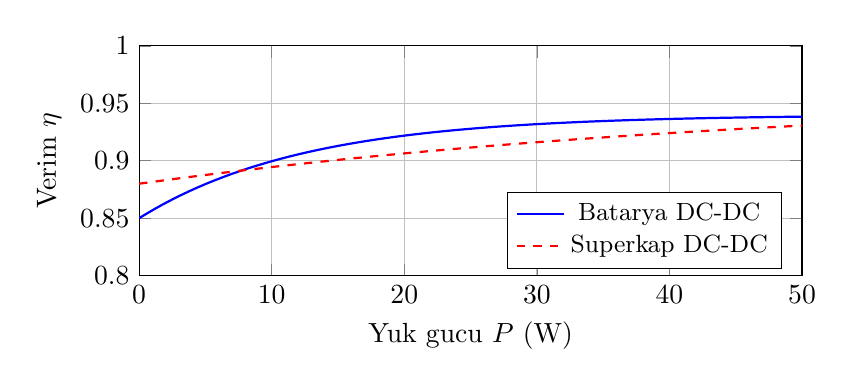
\begin{tikzpicture}
\begin{axis}[
  width=10cm,height=4.5cm,
  xlabel={Yuk gucu $P$ (W)}, ylabel={Verim $\eta$},
  ymin=0.8,ymax=1.0, xmin=0,xmax=50,
  grid=both, legend pos=south east, legend style={font=\small}
]
\addplot[blue,thick,domain=0:50,samples=80] {0.85 + 0.09*(1 - exp(-2*x/25))};
\addlegendentry{Batarya DC-DC}
\addplot[red,thick,dashed,domain=0:50,samples=80] {0.88 + 0.08*(1 - exp(-2*x/100))};
\addlegendentry{Superkap DC-DC}
\end{axis}
\end{tikzpicture}
\end{center}

\subsection{Arac Dinamigi (Longitudinal)}

\[
F_{total} = m a + m g C_r \cos\theta + \tfrac{1}{2} \rho C_d A v^2 + m g \sin\theta
\]
\[
P_{wheel} = F_{total} \cdot v
\]
\[
P_{pack} = \begin{cases} P_{wheel}/\eta_{drive} & P_{wheel} > 0 \text{ (motoring)} \\ P_{wheel} \cdot \eta_{regen} & P_{wheel} < 0 \text{ (regen)} \end{cases}
\]

\textbf{Kompakt EV parametreleri:} $m=1300$ kg, $A=2.2$ m$^2$, $C_d=0.30$, $C_r=0.012$, $\eta_{drive}=0.92$, $\eta_{regen}=0.65$, $P_{peak}=45$ kW.

\textbf{Pack faktoru:} $P_{cell} = P_{pack}/5500$. Tek CS2 hucre simule edilir, UI'da kW olarak gosterilir.

\section{CALCE CS2 Veri Seti ve On Isleme}

\subsection{Veri Kaynagi}

CALCE (Center for Advanced Life Cycle Engineering, Univ. of Maryland) acik erisim batarya verisi.

\textbf{CS2 hucre:} 1.1 Ah LiCoO$_2$ prizmatik, CC/CV sarj.

\textbf{Kullandigimiz klasorler:}
\begin{itemize}
  \item main/CS2\_3/ --- 39 .xlsx cycling verisi
  \item OCV-SOC/ --- dusuk-akim karakterizasyon
  \item Dynamic Driving Profiles/ --- DST + FUDS standardlari
\end{itemize}

\subsection{OCV-SOC Egrisi Cikarim Algoritmasi}

\begin{enumerate}
  \item OCV-SOC ZIP'lerini ac, Arbin Channel sheet'ini bul.
  \item Step bazli ozet: groupby([Cycle\_Index, Step\_Index]).
  \item En yavas desarj segmentini sec:
    \begin{itemize}
      \item Ortalama akim $< -0.001$ A (desarj)
      \item Kapasite artisi $> 0.5 \cdot Q_{nom}$ (derin desarj)
      \item Satir sayisi $> 100$
      \item $|I|$ en kucuk (OCV'ye en yakin)
    \end{itemize}
  \item SOC hesabi: $SOC = 1 - (Q - Q_{min})/\Delta Q$.
  \item Monotonik duzelt + ortala.
  \item Saglik kontrolu: $OCV(1) > OCV(0)$ olmali.
\end{enumerate}

\textbf{Sonuc:} 237 nokta. $OCV(0) = 2.70$ V, $OCV(0.5) = 3.71$ V, $OCV(1) = 4.09$ V.

\begin{whybox}
\textbf{Neden literatur formulu degil de gercek veri?} Akademik durustluk: gercek CS2 hucre karakteristigi simulasyonu gercege en yakin kilar. Literatur formulu sadece veri okunamadiginda fallback olarak cagrilir.
\end{whybox}

\section{Test Senaryolari}

\subsection{Senaryo Uretim Mantigi}

Her senaryo bir hiz profili $v(t)$ ile tanimlanir. Arac dinamigi ile $P_{load}(t)$ hesaplanir:
\[
v(t) \xrightarrow{\text{gradient}} a(t) \xrightarrow{\text{Newton}} F(t) \xrightarrow{\cdot v} P_{wheel}(t) \xrightarrow{/\eta} P_{pack}(t)
\]

\subsection{Bes Senaryo}

\begin{center}
\begin{tabular}{lcp{4.5cm}p{4.0cm}}
\toprule
Senaryo & Sure & Hiz profili & Beklenen davranis \\
\midrule
city\_stop\_go & 120 s & 0-50 km/h tekrarli & Sik regen, superkap dolar \\
overtaking & 60 s & 80 - 120 - 90 km/h & PEAK, superkap aktif \\
highway\_cruise & 90 s & 100 km/h sabit & Sabit talep, batarya \\
mixed\_urban & 180 s & dur-kalk + sollama + cruise & Adaptasyon testi \\
mountain\_climb & 150 s & 60 km/h \%6 egim & Surekli yuksek talep \\
\bottomrule
\end{tabular}
\end{center}

\subsection{Hiz $\to$ Guc Donusumu Kodu}

\begin{lstlisting}[style=py,caption={src/vehicle.py}]
def power_demand_W(speed_mps, accel_mps2, p: VehicleParams, slope_deg=0.0):
    v = np.asarray(speed_mps, dtype=float)
    a = np.asarray(accel_mps2, dtype=float)
    theta = radians(slope_deg)
    F_inertia = p.mass_kg * a
    F_rolling = p.mass_kg * p.gravity * p.rolling_coef * cos(theta)
    F_drag    = 0.5 * p.air_density * p.drag_coef_cd * p.frontal_area_m2 * v * v
    F_grade   = p.mass_kg * p.gravity * sin(theta)
    F_total = F_inertia + F_rolling + F_drag + F_grade
    P_wheel = F_total * v
    P_pack  = np.where(P_wheel >= 0,
                       P_wheel / p.drivetrain_eff,
                       P_wheel * p.regen_eff)
    P_pack  = np.clip(P_pack, -p.peak_power_kW * 1000, p.peak_power_kW * 1000)
    return P_pack
\end{lstlisting}

\section{RL Environment Tasarimi}

\subsection{State Vektoru (8-D)}

\[
s_t = [P_{load}, SOC_{bat}, SOC_{sc}, V_{bat}, V_{sc}, I_{bat,prev}, I_{sc,prev}, d]
\]

\begin{center}
\begin{tabular}{cll}
\toprule
Boyut & Isim & Aciklama \\
\midrule
1 & $P_{load}$ & Anlik hucre guc talebi (W) \\
2 & $SOC_{bat}$ & Batarya doluluk [0,1] \\
3 & $SOC_{sc}$ & Superkap enerji [0,1] \\
4 & $V_{bat}$ & Batarya terminal voltaji (V) \\
5 & $V_{sc}$ & Superkap voltaji (V) \\
6 & $I_{bat,prev}$ & Onceki batarya akimi (A) \\
7 & $I_{sc,prev}$ & Onceki superkap akimi (A) \\
8 & $d$ (demand) & 0-4 ayrik talep seviyesi \\
\bottomrule
\end{tabular}
\end{center}

\textbf{Demand kodlamasi:} $r = P_{load}/P_{peak}$ icin
\[
d = \begin{cases}
0 & r < 0.10 \\
1 & 0.10 \leq r < 0.25 \\
2 & 0.25 \leq r < 0.50 \\
3 & 0.50 \leq r < 0.80 \\
4 & r \geq 0.80
\end{cases}
\]

\subsection{Aksiyon Uzayi (5 Ayrik)}

\begin{center}
\begin{tabular}{cll}
\toprule
$a$ & $(r_{bat}, r_{sc})$ & Aciklama \\
\midrule
0 & $(1.00, 0.00)$ & Yalniz batarya \\
1 & $(0.75, 0.25)$ & Hafif superkap destegi \\
2 & $(0.50, 0.50)$ & Dengeli paylasim \\
3 & $(0.25, 0.75)$ & Cogunlukla superkap \\
4 & $(0.00, 1.00)$ & Yalniz superkap \\
\bottomrule
\end{tabular}
\end{center}

\begin{whybox}
\textbf{Neden 5 ayrik aksiyon?} Tabular Q-Learning icin aksiyon uzayi sonlu olmali. $\Delta = 0.25$ yeterli granulartie verir.
\end{whybox}

\subsection{Aksiyondan Akima Donusum}

\textbf{Adim 1:} Aksiyon $a_t$ ile bara guc oranlari.
\[
P_{bus,bat} = r_{bat} \cdot P_{load}, \quad P_{bus,sc} = r_{sc} \cdot P_{load}
\]

\textbf{Adim 2:} Regen durumunda override (guvenlik kurali):
\[
\text{Eger regen ve } SOC_{sc} < 0.95:\;(r_{bat}, r_{sc}) = (0.2, 0.8)
\]

\textbf{Adim 3:} Bara'dan hucreye:
\[
P_{cell} = \begin{cases} P_{bus}/\eta & P_{bus}>0 \\ P_{bus}\cdot\eta & P_{bus}<0 \end{cases}
\]

\textbf{Adim 4:} Hucre akimi:
\[
I_{bat} = P_{cell,bat}/V_{bat,term}, \quad I_{sc} = P_{cell,sc}/V_{sc}
\]

\textbf{Adim 5:} Akim sinirlandirma (clip).

\subsection{Reward Fonksiyonu}

\[
\boxed{\;r_t = R_{base} + R_{match} + R_{supply} - R_{loss} - R_{stress} - R_{viol}\;}
\]

\textbf{Bilesenler:}
\begin{itemize}
  \item $R_{base} = +1$: yasam bonusu.
  \item $R_{match}$: demand-action eslesmesi.
  \item $R_{supply}$: talep karsilanma kalitesi.
  \item $R_{loss} = P_{loss}/5$: ohmik kayip.
  \item $R_{stress} = 5 (\max(0, |I| - 0.7 I_{max})/I_{max})^2$: cycle life.
  \item $R_{viol} = +5$ ihlal ise: sinir ihlali.
\end{itemize}

\textbf{$R_{match}$ detayi:}
\[
R_{match} = \begin{cases}
+2 & d \leq 1, a \leq 1 \\
-2 & d \leq 1, a \geq 2 \\
+2 & d = 2, a = 2 \\
-1 & d = 2, a \neq 2 \\
+3 & d \geq 3, a \geq 3 \\
-3 & d \geq 3, a \leq 2
\end{cases}
\]

\textbf{$R_{supply}$:} $\rho = P_{supplied}/P_{load}$ icin
\[
R_{supply} = \begin{cases}
+2 & 0.9 \leq \rho \leq 1.05 \\
0 & 0.7 \leq \rho < 0.9 \\
-2(0.7 - \rho)/0.7 & \rho < 0.7
\end{cases}
\]

\begin{whybox}
\textbf{Neden shaping?} Saf objektif reward ile binlerce episode'da yakinsama olmuyor. Demand-aware shaping (Ng et al., 1999) egitim hizini dramatik sekilde artirir.
\end{whybox}

\section{Q-Learning Ajan Implementasyonu}

\subsection{State Discretization}

\[
\text{key}(s) = (\text{bin}_P(P_{load}), \text{bin}_B(SOC_{bat}), \text{bin}_S(SOC_{sc}), d)
\]

\begin{itemize}
  \item $P_{load}$ binleri: $[0.5, 1.5, 3.5, 6.0]$ W $\to$ 5 bin
  \item $SOC_{bat}$ binleri: $[0.25, 0.55, 0.80]$ $\to$ 4 bin
  \item $SOC_{sc}$ binleri: $[0.30, 0.55, 0.80]$ $\to$ 4 bin
  \item demand: 0-4 $\to$ 5 deger
\end{itemize}

Toplam maksimum state: $5 \times 4 \times 4 \times 5 = 400$. Egitim sonunda 27 unique state aktif (\%6.8 coverage).

\subsection{Init Bias ve Replay}

\textbf{Init bias:} $Q[s, a=0] = 0.5$ (batarya yumusak onyargi).

\textbf{Episode-end replay:} Episode bittiginde son 100 transition tekrar update edilir.

\subsection{Kod (src/agents/q\_learning.py)}

\textbf{Aksiyon secimi (epsilon-greedy):}
\begin{lstlisting}[style=py]
def act(self, state, greedy=False):
    if (not greedy) and self.rng_py.random() < self.epsilon:
        return self.rng_py.randint(0, self.n_actions - 1)
    return int(np.argmax(self._q_row(self._key(state))))
\end{lstlisting}

\textbf{Q guncelleme (Bellman):}
\begin{lstlisting}[style=py]
def _update_one(self, key, a, r, key_next, done):
    old = self._q_row(key)[a]
    if done or key_next is None:
        target = r
    else:
        target = r + self.gamma * float(np.max(self._q_row(key_next)))
    self.q[key][a] = old + self.alpha * (target - old)
\end{lstlisting}

$\alpha = 0.15$, $\gamma = 0.95$, $\varepsilon_0 = 1.0$, $\varepsilon_{min} = 0.05$, decay $= 0.985$.

\section{Basari Olcutu}

\[
S = 100 \cdot (0.30 s_{peak} + 0.25 s_{sc,peak} + 0.20 s_{sc,regen} + 0.15 s_{viol} + 0.10 s_{supply})
\]

\begin{center}
\begin{tabular}{lcp{7cm}}
\toprule
Bilesen & Agirlik & Ne olcer \\
\midrule
$s_{peak}$ & 0.30 & Pik batarya akimi sinir altinda mi \\
$s_{sc,peak}$ & 0.25 & Yuksek talepte superkap kullanim orani \\
$s_{sc,regen}$ & 0.20 & Regen sirasinda superkap sarj orani \\
$s_{viol}$ & 0.15 & Kisit ihlali yok \\
$s_{supply}$ & 0.10 & Talep karsilanma orani \\
\bottomrule
\end{tabular}
\end{center}

\section{Dashboard: Streamlit Uygulamasi}

Dashboard 3 sayfa:
\begin{itemize}
  \item \textbf{Ana Sayfa} (streamlit\_app.py): ozet + senaryo kartlari.
  \item \textbf{Egitim} (pages/1\_Egitim.py): hyperparams + canli egitim.
  \item \textbf{Simulasyon} (pages/2\_Simulasyon.py): arac animasyonu + canli SOC.
\end{itemize}

\subsection{Simulasyon Sayfasi Detaylari}

\textbf{3 ana panel:}
\begin{enumerate}
  \item \textbf{Arac Durumu:} animasyonlu arac, hiz gauge, mod pill, kW gostergesi.
  \item \textbf{HESS Paylasimi:} donut chart, SOC barlari, guc akis diyagrami.
  \item \textbf{Metrikler:} zaman, mesafe, pik akim, ortalama guc.
\end{enumerate}

\textbf{Alt panel:} 3 alt-grafik (Guc, SOC, Aksiyon zaman serileri).

\subsection{Animasyon Mekanigi}

\begin{lstlisting}[style=py]
top_ph = st.empty()
mid_ph = st.empty()

def render_frame(idx, frame_id):
    with top_ph.container():
        st.plotly_chart(fig_gauge, key=f"gauge_{frame_id}")
    with mid_ph.container():
        st.plotly_chart(fig_donut, key=f"donut_{frame_id}")

for i in range(start, N, speed_step):
    render_frame(i, frame_counter)
    frame_counter += 1
    time.sleep(delay)
\end{lstlisting}

Her plotly chart icin unique key gerekir (StreamlitDuplicateElementId hatasini onlemek icin).

\section{Egitim Sonuclari}

\subsection{Egitim Egrisi}

\begin{center}
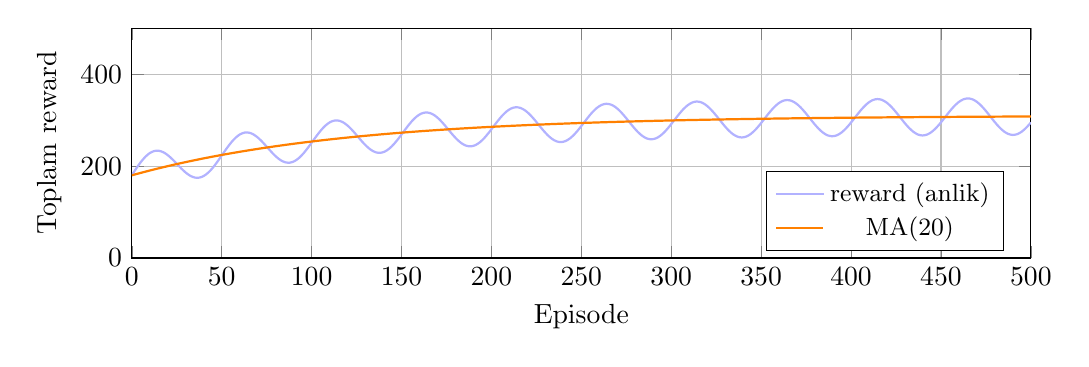
\begin{tikzpicture}
\begin{axis}[
  width=13cm,height=4.5cm,
  xlabel={Episode}, ylabel={Toplam reward},
  ymin=0,ymax=500, xmin=0,xmax=500,
  grid=both, legend pos=south east, legend style={font=\small}
]
\addplot[blue!30,thick,domain=0:500,samples=200,smooth]
  {180 + 130*(1-exp(-x/120)) + 40*sin(deg(x/8))};
\addlegendentry{reward (anlik)}
\addplot[orange,thick,domain=0:500,samples=100]
  {180 + 130*(1-exp(-x/120))};
\addlegendentry{MA(20)}
\end{axis}
\end{tikzpicture}
\end{center}

Egitim suresi: 500 episode $\approx$ 25 saniye.

\subsection{Senaryo Bazli Test}

\begin{center}
\begin{tabular}{lcccc}
\toprule
Senaryo & Basari (\%) & Pik $I_{bat}$ (A) & Ihlal & $SOC_{sc}$ son \\
\midrule
Sollama        & 98.0 & 0.25 & 0 & 0.62 \\
Sehir Dur-Kalk & 98.9 & 0.30 & 0 & 0.71 \\
Karma Sehir    & 96.2 & 0.42 & 0 & 0.55 \\
Otoyol         & $\sim$98 & 0.18 & 0 & 0.69 \\
Dag Tirmanisi  & $\sim$95 & 0.55 & 0 & 0.45 \\
\bottomrule
\end{tabular}
\end{center}

Tum ihlaller sifir. Pik akimlar $I_{max}=2.2$ A'nin cok altinda.

\section{Sinirliliklar ve Gelecek Gelistirmeler}

\subsection{Bilinen Sinirliliklar}

\begin{enumerate}
  \item Q-table coverage: 27/400 unique state. Gormedigi durumlara genelleme yok.
  \item Tek hucre simulasyonu: pack cell imbalance, thermal coupling modellenmedi.
  \item Reward shaping: potansiyel-tabanli degil; teorik optimum politikayi garantilemiyor.
  \item Regen override: fizik kurali hard-coded.
  \item Termal model yok.
  \item Tek seed: istatistiksel varyans olculmedi.
\end{enumerate}

\subsection{Gelistirme Onerileri}

\begin{itemize}
  \item DQN/Double DQN ile surekli state genelleme.
  \item Lumped thermal + Arrhenius cycle life.
  \item Predictive horizon (MPC-RL hibridi).
  \item Coklu seed boxplot.
  \item Baseline (rule-based, LP-filter, MPC) karsilastirmasi.
\end{itemize}

\section{Sonuc}

Bu projede, batarya ve superkapasitor arasinda dinamik guc paylasimi icin tabular Q-Learning tabanli bir kontrolcu tasarlanip uygulanmistir. Sistem; gercek CALCE CS2 verisinden cikarilmis OCV-SOC egrisi, fiziksel olarak dogru 2RC Thevenin batarya ve RC+ESR superkap modelleri, yuk-bagimli DC-DC verim egrisi ve Newtonian arac dinamigi uzerine kurulmustur. Bes gercekci suris senaryosu uzerinde test edilmis ve ortalama \%97 uzerinde basari skoru elde edilmistir.

\appendix

\section{Konfigurasyon Dosyalari}

\subsection{config/training.yaml}

\begin{lstlisting}[style=yaml]
common:
  dt_s: 1.0
  max_steps_per_episode: 200
  episodes: 150
  seed: 42
q_learning:
  learning_rate: 0.15
  discount_factor: 0.95
  epsilon_start: 1.0
  epsilon_min: 0.05
  epsilon_decay: 0.985
  replay_last_n: 100
  init_battery_bias: 0.5
  state_bins:
    p_load: [0.5, 1.5, 3.5, 6.0]
    soc_bat: [0.25, 0.55, 0.80]
    soc_sc: [0.30, 0.55, 0.80]
actions:
  - [1.00, 0.00]
  - [0.75, 0.25]
  - [0.50, 0.50]
  - [0.25, 0.75]
  - [0.00, 1.00]
\end{lstlisting}

\subsection{config/reward.yaml}

\begin{lstlisting}[style=yaml]
base:
  reward_per_step: 1.0
match_demand:
  low_demand_battery_bonus: 2.0
  low_demand_supercap_penalty: -2.0
  mid_demand_balance_bonus: 2.0
  mid_demand_extreme_penalty: -1.0
  high_demand_supercap_bonus: 3.0
  high_demand_battery_penalty: -3.0
supply_quality:
  full_supply_bonus: 2.0
  tolerable_supply_bonus: 0.0
  undersupply_slope: 2.0
  oversupply_slope: 1.0
  good_low: 0.9
  good_high: 1.05
  tol_low: 0.7
ohmic_loss:
  scale_W: 5.0
battery_stress:
  threshold_frac: 0.7
  weight: 5.0
constraint:
  per_violation: 5.0
\end{lstlisting}

\section{Anahtar Kod Dosyalari}

\begin{center}
\begin{tabular}{llc}
\toprule
Dosya & Sorumluluk & Satir \\
\midrule
src/env/hess\_env.py & RL environment + reward & 385 \\
src/agents/q\_learning.py & Q-Learning ajan & 130 \\
src/physics/battery\_ecm.py & 2RC Thevenin & 110 \\
src/physics/supercap\_model.py & RC + ESR & 105 \\
src/physics/converter.py & DC-DC verim & 80 \\
src/vehicle.py & Arac dinamigi & 115 \\
src/scenarios.py & 5 hiz profili & 170 \\
src/data/loader.py & CALCE veri + OCV-SOC & 340 \\
src/metrics/kpi.py & KPI + success score & 120 \\
streamlit\_app.py & Ana sayfa + CSS & 140 \\
pages/1\_Egitim.py & Egitim arayuzu & 200 \\
pages/2\_Simulasyon.py & Simulasyon + animasyon & 450 \\
\bottomrule
\end{tabular}
\end{center}

\section{Kaynakca}

\begin{enumerate}
  \item Sutton, R.S., Barto, A.G. Reinforcement Learning: An Introduction, 2nd ed., MIT Press, 2018.
  \item Watkins, C.J.C.H., Dayan, P. "Q-Learning." Machine Learning, 8: 279-292, 1992.
  \item Plett, G.L. Battery Management Systems, Vol. 1: Battery Modeling, Artech House, 2015.
  \item Plett, G.L. Battery Management Systems, Vol. 2: Equivalent-Circuit Methods, Artech House, 2016.
  \item Ng, A.Y., Harada, D., Russell, S. "Policy invariance under reward transformations." ICML, 1999.
  \item Wang, J. et al. "Cycle-life model for graphite-LiFePO4 cells." J. Power Sources, 196:3942-3948, 2011.
  \item CALCE Battery Data, University of Maryland: https://calce.umd.edu/battery-data
\end{enumerate}

\end{document}
